\documentclass[../report.tex]{subfiles}
\graphicspath{{\subfix{../image/}}}

\begin{document}
% Intro start
% Flavour text as an intro short
% Mindmap 
% Brief description of the mindmap
% Forklift was chosen shortly 

\subsubsection{Introduction - Why a forklift?}
    Throughout history a certain industrial trend has become the most pronounced 
    it has ever been, automation. Any and all tasks that could be automated in a
    financially viable way have seen at least one instance of it happening. This
    is due to the numerous benefits that an autonomous system can provide. In a
    similar vein our team also aimed at contributing to this phenomenon within 
    the scope of the third semester project. The aim of the project was to make
    an autonomous intelligent vehicle.

    Project work started with exploring the possible fields where such a vehicle
    could find sensible applications. This mindmap portrays the various ideas considered. 
    Some of these include a food and beverage delivery system both in a restaurant and home
    settings and some were related to various monitoring systems. Others had more a focus
    on everyday home-support.

    \begin{figure}[H]
        \centering
        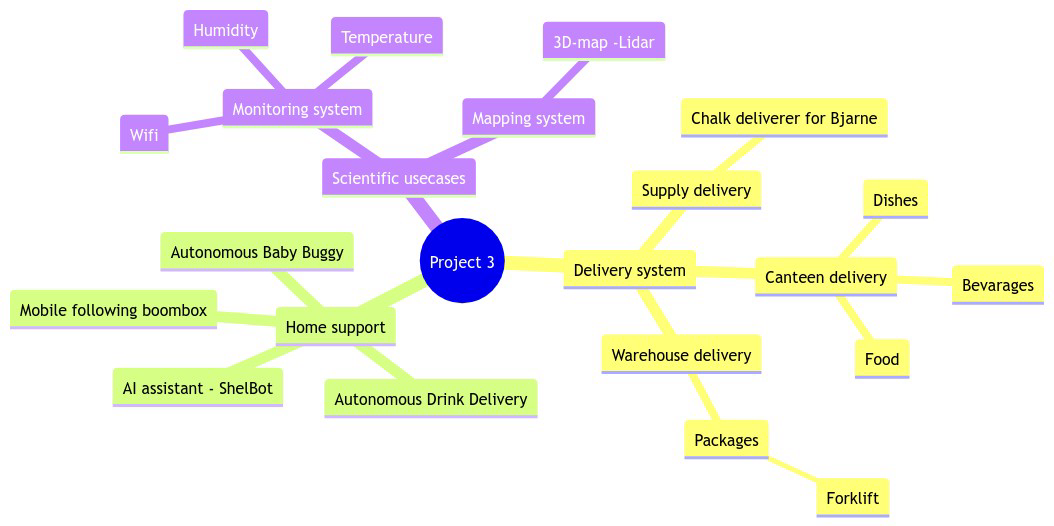
\includegraphics[width=0.8\linewidth]{MindmapProjectOptions.md.1.png}
        \caption{Mind-map of project ideas}
    \end{figure}   

    Throughout the idea phase, the aspect of presenting the idea at the tech
    expo at the end of the semester was important. The audience should be able
    to grasp the concept of the project and understand how it could be
    beneficial in everyday life.
\end{document}